\section{Method}
The general idea is similar to generating the medial axis transform and round the distance measures,
such that an exact integer beads will fit the polygon there
so that there is never a gap region left over in the middle of the polygon.

We round to integer multiples of half the nozzle width so as to allow single-bead segments, rather than only having polygonal insets.

\begin{figure}
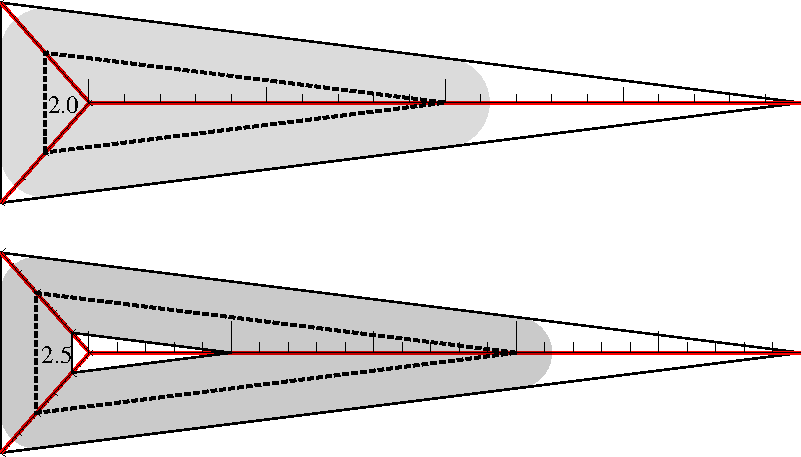
\includegraphics[width=\columnwidth]{sources/method/rounded_vs_unrounded.pdf}
\caption{Toolpaths employing dist rounding vs without.}
\label{rounded_vs_unrounded}
\end{figure}


\subsection{Method Overview}
The global idea is that we locally decide on the number of beads everywhere in the input shape, then apply a beading strategy to determine the widths of the beads and then generate the toolpath locations and widths from this.
We decide on a bead count at locations which lie in the middle of the shape in some sense to be defined.
The beading strategy then gives us the beading widths and locations in between those center locations and the outline.
These beadings are then used to generate the toolpath junctions, which are connected together to form the extrusion toolpaths with varying width.

\begin{enumerate}
\item Compute a skeletonization of the outline shape based on the Voronoi diagram.
\item Use a significance measure to mark portions of the skeleton which lie in the center.
\item Determine the bead count values in the significant regions and handle transitions to different bead count values.
\item Generate ticks along insignificant bones of the skeleton and connect the ticks together to extract the toolpaths.
\end{enumerate}


\hl{Idea: generate only outer 3 walls, except in significant regions where the distance $R < 5 \win$, so as to prevent jagged infill lines.}
\Cref{wedge_and_infill}

\hl{Filter beading number in order to prevent regions with a lot of back and forth transitions.}

\subsection{Terminology}
For an explanation of the terms used, see \cref{legend}.

\begin{figure}
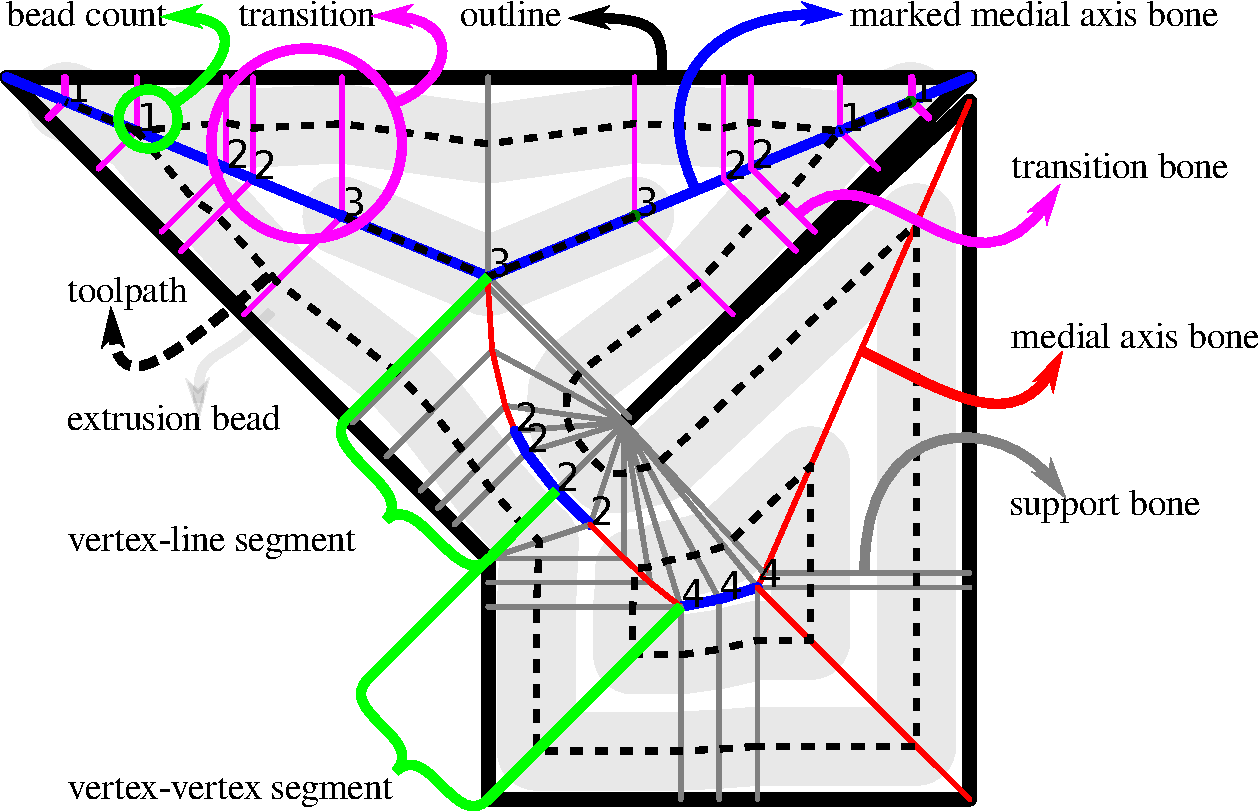
\includegraphics[width=\columnwidth]{sources/method/terminology.pdf}
\caption{Explanation of terms.}
\label{legend}
\end{figure}



\hl{We need consistent terminology and symbols which adhere to standards in literature.}
The following synonym groups are used here which are not yet checked with existing literature':
\begin{itemize}
\item bones, skeleton segment
\item joints, ticks, vertices, locations
\item feature radius $R$, $\nicefrac12$ total distance $d$
\end{itemize}


Based on the straight skeleton naming, I would like to introduce a new consistent terminology:
\begin{itemize}
\item any skeleton segment: bone
\item skeleton vert: joint
\item location of an insets along a bone: tick
\end{itemize}






















\subsection{Skeletonization}
In order to apply the beading strategy to an arbitrary outline polygon we look at the skeleton of the polygon.
There are several possible skeletonal structures we could consider.


\subsubsection{Background}
One of the most commonly used skeletonizations of a shape is the medial axis.
The medial axis is defined by the locations where the inscribed circle meets the boundary in at least two locations. \todo{[citation needed]}
See \cref{MAT_explanation}.

``Because of its shape, the medial axis of a figure is also called the skeleton or the symmetric axis of the figure.
Associated with the medial axis is a radius function $R$, which defines for each point on the axis its distance to the boundary of the object.''
\cite{lee1982medial}

The medial axis along with the feature radius combine into a complete feature decsriptor, called the medial axis transform (MAT).
The MAT can unambiguously recreate the input shape exactly. \todo{[citation needed]}

\cite{Moesen2011} provides a thorough overview of all MAT algorithms.
\cite{Moesen2011} calls $R$ the `feature radius': ``In every point $p \in P$, and thus also in points on the MA, the feature radius $\text{rad}(p)$ of $p$ can be defined as the Euclidean distance to the closest point on the boundary of $P$.''


\begin{figure}
\centering
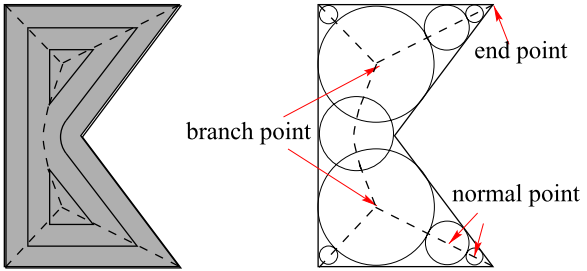
\includegraphics[width=.9\columnwidth]{sources/intro/medial_axis_Kao.png}
\caption{MAT explanation by \citeauthor{kao1998optimal}}
\label{MAT_explanation}
\end{figure}


\begin{figure}
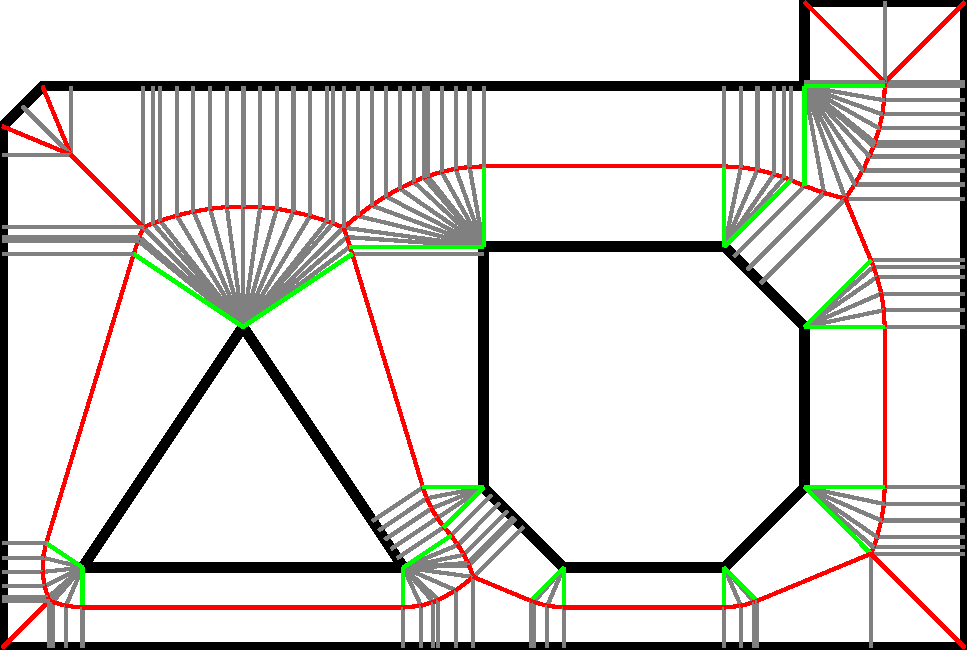
\includegraphics[width=\columnwidth]{sources/method/MAT_VD_VQ.pdf}
\caption{
Skeletonization of an outline shape (black).
Relation between the medial axis (red), the limited Voronoi Diagram (red and green) and the Voronoi Quadrangulation (red, green and gray): MAT $\subset$ Limited VD $\subset$ VQ.
}
\label{skeletonization_comparison}
\end{figure}



\subsubsection{Voronoi Quadrangulation}
\todo{The Voronoi Quadrangulation has already been described in} \cite{Ding2016a}. Section 2.4 Domain Decomposition.

The medial axis of a polygonal shape can be obtained from the Voronoi Diagram (VD) generated on the line segments and vertices of the shape. \cite{lee1982medial}
First we throw away all locations in the Voronoi diagram which fall outside the boundary shape.
We can then obtain the medial axis by further reducing the Voronoi bones connected to a concave corner in the boundary shape.

However, instead of removing bones from the Voronoi diagram we will introduce more bones such that the skeleton discretizes the boundary shape into quads within which the $R$ can be interpolated linearly.
We call the resulting skeletonization the \emph{Voronoi Quadrangulation} (VQ).
See \cref{skeletonization_comparison}.
The VQ greatly simplifies the processing required downstream in our framework.

In order to generate the VQ, we start by generating a normal Voronoi Diagram and remove all segments which lie outside of the boundary shape.
We then introduce bones such that each node in the VQ is directly connected to the outline via a single bone:
each node in the VQ is connected to the closest points on the boundary (its \emph{support}).
As such the VQ divides the polygon in quads consisting of 1 outline segment and 3 bones, one of which is not directly connected to the outline.
However some of these quads are triangles, as can be seen in \cref{discretization}.

We then also discretize parabolic bones and bones generated by two concave outline vertices into approximately equidistant segments.
See \cref{discretization}.
That way we can approximate the feature radius $R$ in between two nodes $v_0$ and $v_1$ in the VQ by interpolating linearly between $R(v_0)$ and $R(v_1)$.
Furthermore, we can linearly interpolate the distance field of a quad $p_0v_0v_1p_1$ (where $p_0$ and $p_1$ lie on the outline shape):
For a point $a \in p_0v_0$ and a point $b \in p_1v_1$ for which $R(a) = R(b)$ we have that all points in the line segment $ab$ have the same feature radius $R$.

\begin{figure}
\centering
%\begin{subfigure}{0.45\textwidth}
%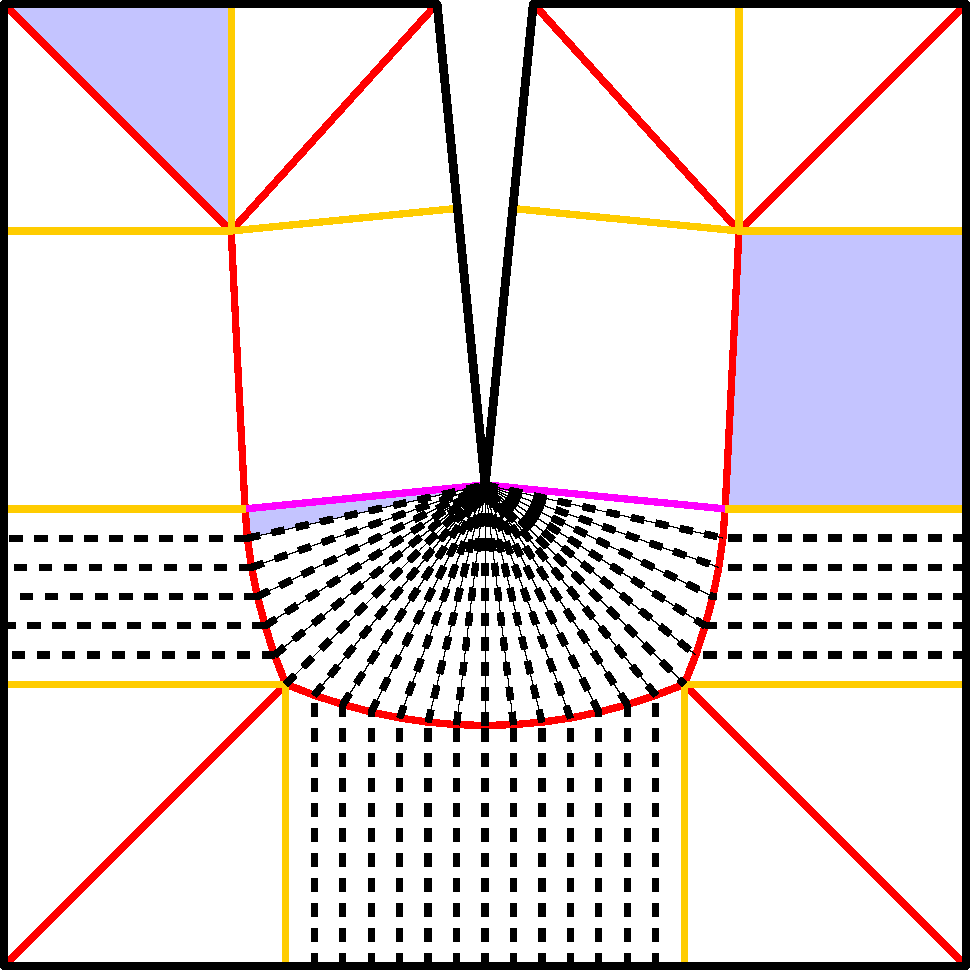
\includegraphics[width=\columnwidth]{sources/method/parabola_dip.pdf}
%\caption{asf}
%\end{subfigure}
%\begin{subfigure}{0.45\textwidth}
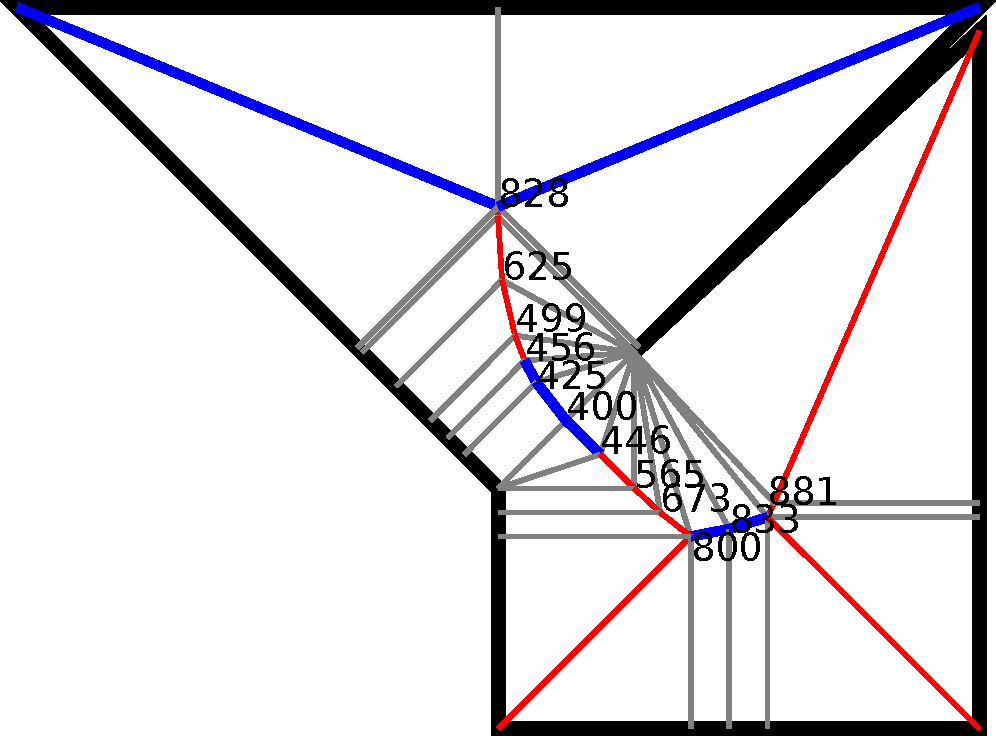
\includegraphics[width=\columnwidth]{sources/method/point-point_and_point-line_segments.pdf}
%\caption{Transitioning}
%\end{subfigure}
\caption{
Voronoi quadrangulation domain decomposition.
Medial axis (red and blue) is augmented with (gray) edges connecting each node to its nearest support points in the outline shape.
Parabolic medial axis segments are discretized and likewise for segments generated by two concave outline vertices, because the feature radius (black text in microns) doesn't increase linearly along those segments.
The blue segments are significant according to $\alpha_\text{max} = 135\degree$.
}
\label{discretization}
\end{figure}



\subsection{Beading}
We assign a bead count to each node in the skeleton which is connected to a bone which is in `the center' of the shape
and also to each node with locally optimal feature radius $R$.
Around regions where the bead count changes we introduce transition regions.


\subsubsection{Significance measure}\label{sec:significance_measure}
Places where the naive concentric toolpathing strategy would create large underfilling and overfilling areas are locations which intuitively look like `the center' of the shape.
This can be formalized by looking at the significance measure knows as the \emph{bisector angle}.
The bisector angle $\alpha$ is the angle $\angle{p_ovp_1}$ between a location $v$ on a bone of the skeleton and its two supporting polygon points $p_0$ and $p_1$. \cite{attali1996modeling}
For a polygon with a pointy wedge area of an angle $\beta$, we have $\alpha = 180\degree - \beta$, which corresponds to overfill areas and underfill areas the size of $\nicefrac12 w^2 \left( \nicefrac14 \tan ( \alpha / 2) - \alpha / 2 \right)$ when filled using a naive strategy of constant bead width $w$.
See \cref{naive_overfill_underfill}.
The bisector angle is therefore an exact measure of the amount of overfill and underfill.
Contrary to related literature we will \emph{keep} the insignificant regions of the skeleton.
Our framework will employ a different toolpathing strategy to prevent overfill and underfill areas if they would be so large that $\alpha > \alpha_\text{max}$.


\begin{figure}
\centering
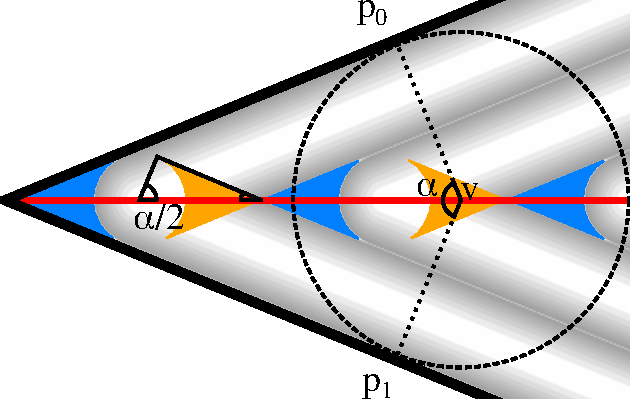
\includegraphics[width=\columnwidth]{sources/method/naive_overfill_underfill.pdf}
\caption{
Overfill and underfill areas in a naive beading using a constant bead witdh $w$ of a wedge area with vertex angle $\beta$.
The underfill areas (light blue) are mirrored versions of the overfill areas (dark red).
The bisector angle $a = 180\degree - \beta$ is the angle between a location $v$ and its support $p_0$ and $p_1$.
}
\label{naive_overfill_underfill}
\end{figure}


A computationally efficient way to compute $\alpha$ can be obtained by looking at the ratio between feature radius $R$ and the Euclidean distance.
if $ | R(v_1) - R(v_0) | / |v_1 - v_0| >  \cos(\alpha_\text{max} / 2)$ then $\alpha > \alpha_\text{max}$.
See \cref{distance_based_angles}.
This ratio can readily be applied to simple skeleton segments to determine whether they are significant.
For skeletal segments generated by a polygon vertex at $(0,d)$ and a line segment through $(0,0)$ and $(0,\epsilon)$ or another vertex $(0,0)$, we can determine the significant portion by evaluating $\frac{\partial R}{\partial x} > \cos(\alpha_\text{max} / 2)$.
For parabolas we introduce extra points in the discretization at the two bounds where $| x | = d  / \tan(\alpha_\text{max} / 2)$
and for bones with vertex-vertex support we introduce discretization points at the two bounds where $| x | = \nicefrac12 d  / \tan(\alpha_\text{max} / 2)$.
This ensures that the discretization doesn't alter the extent and existance of significant regions.

\begin{figure}
\centering
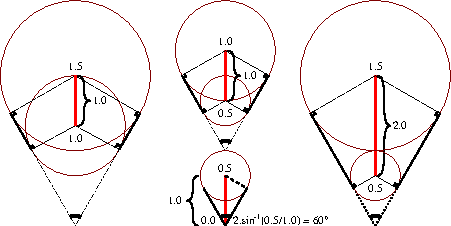
\includegraphics[width=.9\columnwidth]{sources/method/distance_based_angles.pdf}
\caption{
Distance based angle estimation.
By comparing the Euclidean distance between two vertices with the feature radius $R$ we can skip comparing the angles between the outline segments.
}
\label{distance_based_angles}
\end{figure}

The Euclidean distance between two skeletal vertices can never be less than the difference in the feature radius $R$ measure between the vertices: \cref{distance_ratio_limit}.

\begin{figure}
\centering
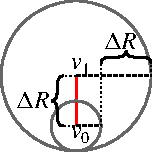
\includegraphics[width=.3\columnwidth]{sources/method/distance_ratio_limit.pdf}
\caption{Minimal Euclidean distance for a given difference in feature radius $R$.}
\label{distance_ratio_limit}
\end{figure}

Any node in the skeleton can have at most two significant bones connected to it, because we have limited $\alpha_\text{max} > 120\degree$,
while the corners of a triangle can only add up to \SI{180}{\degree}.
\todo{TODO: make figure which clearly shows this!}
This results in the fact that we will never have 3-way intersections of non-closed extrusion toolpaths.
(Simple case) If 2 edges of the VQ meet then 3 outline segments are involved; lines through those segments form a triangle which cannot have more than two angles less than \SI{60}{\degree}.
However, what if we connect two significant segments using a small insignificant segment?
There is a distance limit based on \cref{distance_ratio_limit}:
the connecting segment is always larger in Euclidean distance than the difference in feature radius $R$.



\subsubsection{Properties of significant regions}
A node in the graph can have at most two significant edges.
For a node in the VD $v$ with a support of three points on the outline polygon $p_1, p_2, p_3$, the bisector angles $\angle{p_1vp_2} + \angle{p_2vp_3} + \angle{p_3vp_1} = 360\degree$, so if two angles are more than $\alpha_\text{max} > 120\degree$ the third one needs to be smaller than $360\degree - 2\alpha_\text{max} < 120\degree$ and therefore nonsignificant.
% However, because of some filtering operations this property does not neccesarily hold for the markings.
The extra edges added to the VD to form the VQ can never be significant because their bisector angle is \SI{0}{\degree} by definition,
so the nodes of the VQ also have at most two significant edges.

A saddle point is always marked.
When going from one local maximum to another we must pass through a significant region.
You will either go through the marked region of a discretized parabola or of a segment with two polygonal vertices as support.
This menas that the feature radius function in between marked regions is monotonic.
This means that when propagating beadings downward from marked regions they can never conflict in the middle - they will always conflict at either marked region.

From any node in the graph which is not a saddle point there is at most a single edge going upward.
Any branch point $v$ in the VD coincides with the circumcircle of its support $p_1, p_2, p_3$.
If $v$ lies within $\triangle p_1 p_2 p_3$ it is a local maximum and otherwise we will show it has exactly one upward edge.
If $v$ lies outside of $\triangle p_1 p_2 p_3$ then those support points lie within a \SI{180}{\degree} range from $v$
and one point lies in the middle, say $\angle p_1 + \angle p_2 = \angle p_3$.
Then a circle with radius $R(v) + \epsilon$ around $w$ such that $|v-w| < 2 \epsilon$ can only touch $p_1$ and $p_3$.
See \cref{branch_upward_edge_property}.
%See VoronoiQuadrangulation::filterUnmarkedRegions
This means that walking up the graph from a marked region to a local maximum follows a single path without branching.

\begin{figure}
\centering
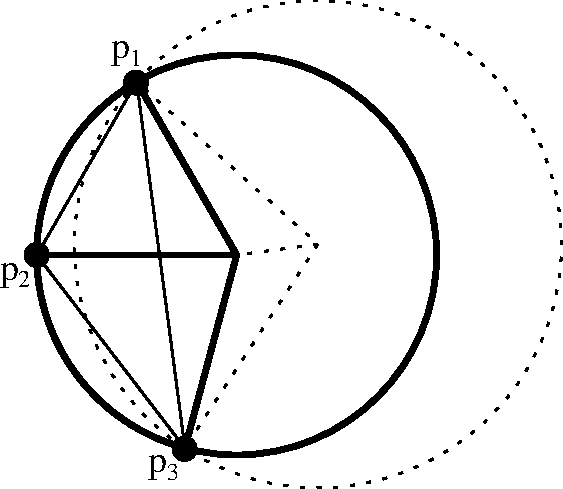
\includegraphics[width=.4\columnwidth]{sources/method/branch_upward_edge_property.pdf}
\caption{The radial distance can only increase along one edge around a branch point in the VD.}
\label{branch_upward_edge_property}
\end{figure}



The two downward edges from a branch point cannot both be significant.
A branch point which is not a local maximum generated by the support points $p_1, p_2, p_3$ has bisector angles such that $\triangle p_1 p_2 p_3$ has its circumcentre $v$ outside of the triangle, because otherwise the feature radius decreases in all directions.
This means that all support points lie within a \SI{180}{\degree} range around the node. 
Suppose the one edge going upward is generated by $p_1$ and $p_3$.
Then the bisector angle $\angle p_1 v p_3 < 180\degree$ and $\angle p_1 v p_2 + \angle p_2 v p_3 < 180\degree$,
so if $\angle p_1 v p_2 < 120\degree$ then $\angle p_2 v p_3 < 60\degree$ and is therefore not significant. 
%so at most either of $\angle p_1 v p_2$ and $\angle p_2 v p_3$ has a significant bisector angle.




\subsubsection{Bead counts}
In order to apply the beading strategy to the VQ
we assign each significant node $v$ of the skeleton a bead count $v.B^*$ which is initialized to $b(R(v))$, but it is modified in order to prevent discontinuities and remaining gaps.

We also assign a bead count $v.B^*=b(R(v))$ to all nodes $v$ which are local maxima, i.e. the $v$ for which $\forall v_\text{n} \in v.\text{neighborhood} : R(v) > R(v_\text{n})$. 
This prevents the single overfill or underfill region in non-significant regions.
See \cref{rounded_vs_unrounded}.




\subsubsection{Transitioning}
In order to prevent discontinuities in the toolpaths around locations where the bead count changes, we need a way to smoothly transition to a different number of beads around locations where the 3D model has a changing radius.
See \cref{transitions}.
The transition will be placed anchored on each location $v$ where $R(v) = \nicefrac12 b^{-1}(n+1)$ for any lower bead count $n$.
At the start $v_0$ and end $v_1$ of the transition we introduce a new node in the skeleton and connect it to the outline as per the VQ requirement.
We then assign $v_0.B^* = n$ and $v_1.B^* = n + 1$.
If there is any node $v_x$ in between $v_0$ and $v_1$ we assign it a fractional bead count by linear interpolation: $v_x.B^* = n + D(v_0, v_x)/t(n)$, where $D(.)$ is the Euclidean distance measured along the significant bone(s).
See \cref{distance_rounding_transition}.



\begin{figure*}
\centering
\begin{subfigure}{0.9\textwidth}
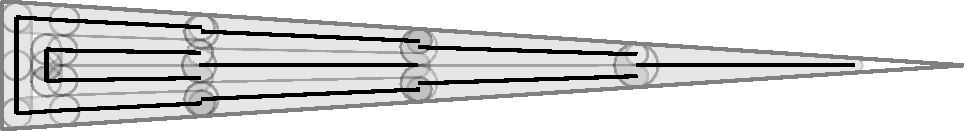
\includegraphics[width=\columnwidth]{sources/method/wedge_distributed_generated__no_transitions.pdf}
\caption{Without transitioning}
\end{subfigure}
\begin{subfigure}{0.9\textwidth}
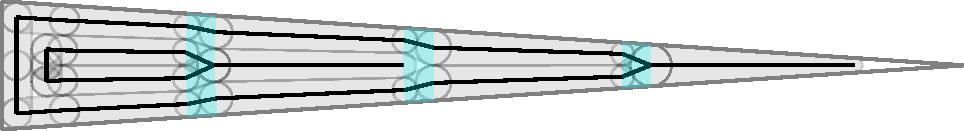
\includegraphics[width=\columnwidth]{sources/method/wedge_distributed_generated.pdf}
\caption{Transitioning}
\end{subfigure}
\caption{
Discontinuities around regions where the bead count changes are prevented by transition regions (highlighted in cyan).
}
\label{transitions}
\end{figure*}

We determined above that $v_0$ and $v_1$ should be placed around $v$, but their exact position has yet to be specified.
While the Euclidean distance between them is $t(n-1)$, the distance between $v_0$ and the anchor point $v$ is yet to be specified.
We determine the distance between the anchor and the transition start $v_0$ proportial to the positioning of the transition relative to the preferred distances: $D(v_0, v) =  t(n) (b^{-1}(n+1) - p(n) ) / (p(n+1) - p(n))$.
That way the transitions never override the preferred beading.
See \cref{transition_placement}.


\begin{figure}
\centering
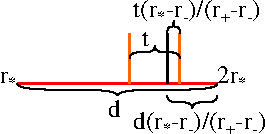
\includegraphics[width=.3\columnwidth]{sources/method/transition_location_precise.pdf}
\caption{
Transition placement.
The anchor position within the transition length is proportional to the transition location within the range between two distances with preferred length. 
}
\label{transition_placement}
\end{figure}


\begin{figure}
\centering
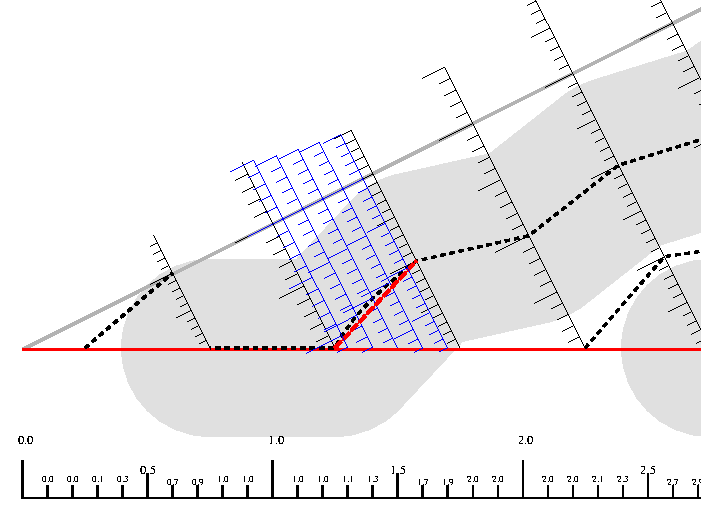
\includegraphics[width=.9\columnwidth]{sources/method/distance_rounding_transition.pdf}
\caption{Feature radius remapping.}
\label{distance_rounding_transition}
\end{figure}


\subsubsection{Transitioning to insignificance}
In significant regions of the VQ we employ the approach of applying the optimal bead counts and employing transitioning, while in insignificant regions the beading is only governed by the beading of locations with locally optimal feature radius.
Significant bones always form chains and don't branch out because of the angle constraint on $\alpha_\text{max}$.
At the end of such chain $v$ we may need to transition from the former approach to the latter.
This only happens when the feature radius continues increasing: if $\exists v_n \in v.\text{neighborhood}: R(v) < R(v_n) \land | R(v) - R(v_n) | / |v - v_n| >  \cos(\alpha_\text{max} / 2)$ then the bead count assigned by the significant region doesn't fit with a beading which would follow from a local optimum at $v_n$ or some farther node.
See \cref{transition_to_insignificance_problem}.


\todo{Applying the bead count and determining the beading with the associated widths $W$ and locations $L$ is only handled in the next section, so perhaps we should introduce the beading propagation before the section on transitioning.}
See \cref{alg_beading_propagation}.

\begin{figure}
\centering
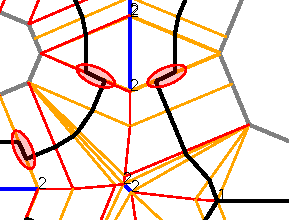
\includegraphics[width=.5\columnwidth]{sources/method/transition_to_insignificance_problem.pdf}
\caption{
Problems at significance boundary regions highlighted with red ovals.
The beading approach from the significant region (blue) results in toolpaths (black) which don't line up with the approach following from the beading which results from the bead count at the center bottom.
}
\label{transition_to_insignificance_problem}
\end{figure}


The transition length of these transitions to insignificance is determined by the fractional difference in bead count between the two beadings:
if $v.B^* < n$ then $t = t(n) . (R(v) - v.L_n)$
otherwise $t = t(n) . (1 - (R(v) - v.L_n))$,
where $n = \argmax_i v.L_i < R(v)$.
At a distance $t$ from $v$ along significant bones we introduce an new node $v_0$ for the end of the transition and again we connect it to the outline as per the VQ requirements.


We modify $v.B^*$ such that it coincides with the beading propagated to $v$ from some farther local optimum or another significant region.
(This propagation is explained in \cref{section_toolpath_extraction}.)
We assign $v.B^* = n + 1 - \epsilon$, so that the transition switches from the significant beading to the beading of the insignificant approach entirely.
For nodes $v_x$ in between $v_0$ and $v$ we interpolate $v_x.B^*$ again linearly based on the Euclidean distance along the bones in between $v$ and $v_0$.

\todo{TODO: implement this! }
\todo{Compute beading propagation after initial $B^*$ assignment, but before transitioning}
\todo{Explain beading propagation before transitioning}












\subsection{Toolpath extraction}
\label{section_toolpath_extraction}



\subsection{Beading strategy}
First we determine how we should fill a 	polygon with constant width with a number of beads.
We want to fit an exact whole number of beads in order to prevent a gap being generated.
We consider only half of the polygon, because our beading strategy should be symmetrical.

We define a beading strategy as the following set:
$$
\left\{ b(d), p(n), W(n, d), L(n, d), t(n), \alpha_{\text{max}} \right\}
$$
where
$b(d)$ gives the optimal bead count to cover a total distance of $d$,
$p(n)$ gives the optimal total distance of a given bead count $n$,
$W(n, d)$ gives the sequence of bead widths to cover a distance $d$ using $n$ beads,
$L(n, d)$ gives the sequence of toolpath positions as distances from the outline to cover a distance $d$ using $n$ beads,
$t(n)$ is the length of the transition region to switch from $n$ to $n+1$ beads
and
$\alpha_{\text{max}}$ is the limit bisector angle of the significance measure.


We call a distance $d$ `preferred' when $d = p(b(d))$
For our method we require the inverse $b^{-1}(n)$ which gives the smallest $d$ for which $b(d) = n$.

The following restrictions hold:
\begin{itemize}
\item $b(d) \geq 0, W(n,d) > 0, L(n, d) \geq 0, t \geq 0$
\item $120\degree < \alpha_{\text{max}} \leq 180\degree$
\item $W$ is symetric: $W(n, d)_i = W(n, d)_{n-i-1}$
\item $L$ is symmetric in $d$: $L(n, d)_i = d - L(n, d)_{n-i-1}$
\item $p$ is within the range of optimal: $b^{-1}(n) < p(n) < b^{-1}(n + 1)$
%\item $b \left( p(n) \right) = n$ % follows from the above!
\item $b$ is monotonic: $ b(d) \leq b(d + \epsilon)$
\item $W_n$ is monotonic and continuous at each bead index $n$ for constant bead count $c$: $0 \leq \frac{\partial W(c, d)_n}{\partial d} < \infty$.
\item $t$ is viable: $t(n) < \left( p(n + 1) - p(n) \right) /{2 \cos \alpha_\text{max}}$
\end{itemize}

The angle requirement ensures that there is never a 3-way junction of significant bones.

By applying the beading strategy to a skeleton location $v$ and a predetermined bead count $n$ we get a beading, which is defined as the following set:
$$
\left\{ d, w_i, l_i  \right\}
$$
where
$d = 2 R(v)$ is the total distance associated with $v$,
$w_i$ is the bead width of the bead with index $i$
end
$l_i$ is the distance of the toolpath location of bead $i$ from the outline.



\subsubsection{Tick placement}
\hl{Change terminology: location $\to$ junction?}

Now that we have the skeleton set up, we determine the locations along the bones where the vertices of the toolpath polygons should be: the \emph{ticks}.
For significant regions we have already inroduced joints around the transitions which serve as those locations.
For insignificant regions we can simply apply the beading strategy in order to find the toolpath verts.


This needs to be stable against small perturbations in the outline polygon.
See \cref{heterogeneous_joint_generation}.
For any sequence on insignificant bones from the outline polygon inward we define the stable end point as the first vertex which is connected to a significant VQ segment.
Based on the feature radius $R$ there we place ticks along the insignificant bones following the beading strategy.

\begin{figure}
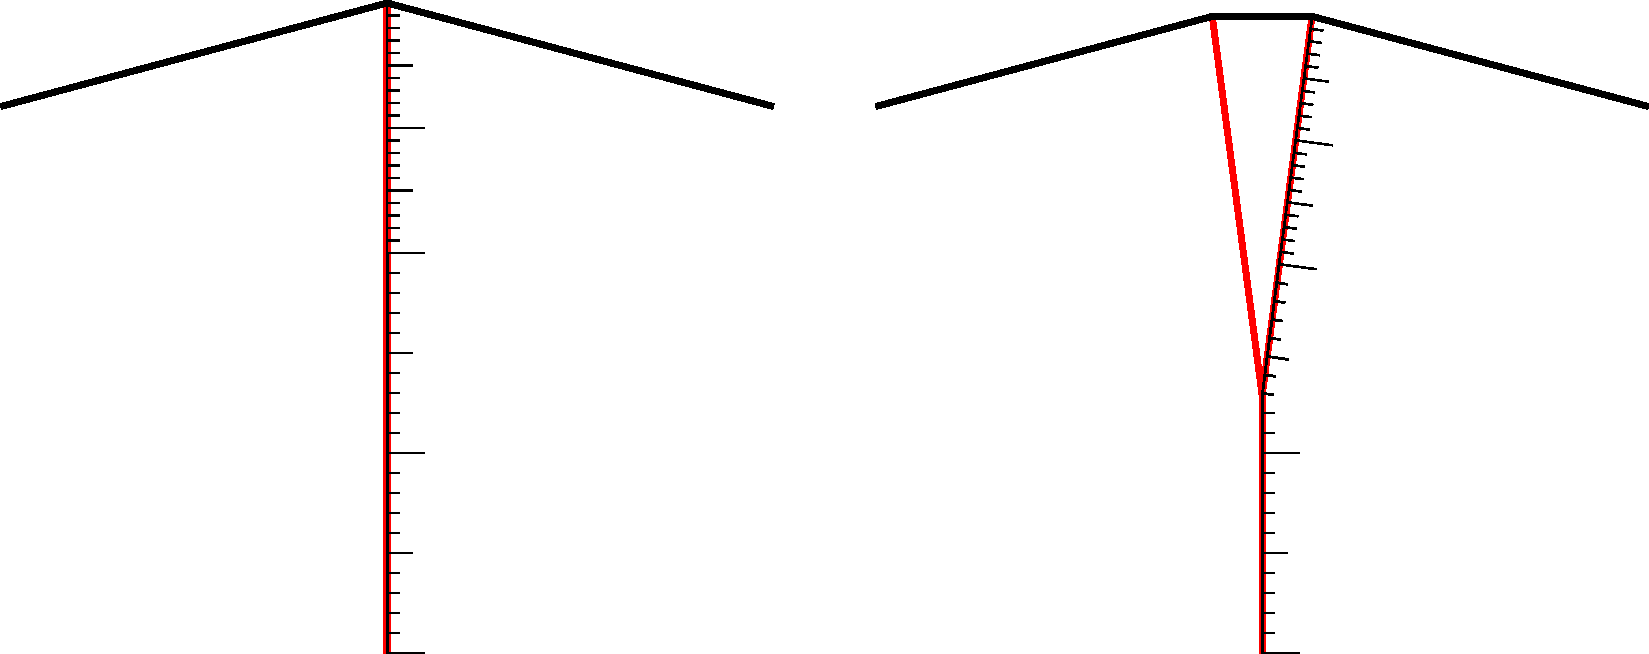
\includegraphics[width=\columnwidth]{sources/method/heterogeneous_joint_generation.pdf}
\caption{Toolpaths employing dist rounding vs without.}
\label{heterogeneous_joint_generation}
\end{figure}





\subsubsection{Toolpath extraction algorithm}
After the beading strategy has been applied we have a beading associated with each significant node as well as each node with locally optimal $R$.
In order to determine the tick locations of quads which don't contain any such node, we propagate the beading information down.
We therefore sort all quads on their highest $R$-value and process the high $R$ quads first.
The beading information is then passed down along the bones of the quad to lower $R$ nodes if those nodes don't already have a beading associated.

See \cref{alg_beading_propagation}.

\begin{algorithm}
\caption{Beading propagation}
\label{alg_beading_propagation}
\begin{algorithmic}
\State quads.sortOn(getHighestR())
\ForAll{$q \in$ quads}
	\State $v_\text{max} = q$.getHighestR()
	\State beading = retrieveBeading($v_\text{max}$)
	\If {$\neg$ retrieveBeading($v_\text{max}$.next())}
		\State storeBeading($v_\text{max}$.next(), beading)
	\EndIf
	\If {$\neg$ retrieveBeading($v_\text{max}$.prev())}
		\State storeBeading($v_\text{max}$.prev(), beading)
	\EndIf
\EndFor
\end{algorithmic}
\end{algorithm}


We can then process all bones in arbitrary order and generate the ticks along those bones.
See \cref{alg_tick_generation}.

\begin{algorithm}
\caption{Tick generation}
\label{alg_tick_generation}
\lstset{language=C++}
\begin{lstlisting}[frame=single]
Point a = edge->to->p;
Point b = edge->from->p;
Point ab = b - a;

int start_R = edge->to->data.distance_to_boundary; // higher R
int end_R = edge->from->data.distance_to_boundary; // lower R
assert(end_R <= start_R);

int junction_idx;
// compute starting junction_idx for this segment
for (junction_idx = (beading->toolpath_locations.size() - 1) / 2; junction_idx >= 0 && junction_idx < beading->toolpath_locations.size(); junction_idx--)
{
  int bead_R = beading->toolpath_locations[junction_idx];
  if (bead_R <= start_R)
    break; // junction coinciding with start node is used in this function call
}

for (; junction_idx >= 0 && junction_idx < coord_t(beading->toolpath_locations.size()); junction_idx--)
{
  int bead_R = beading->toolpath_locations[junction_idx];
  assert(bead_R > 0);
  if (bead_R < end_R)
    break; // junction coinciding with a node is handled by the next segment
  
  Point junction(a + ab * (bead_R - start_R) / (end_R - start_R));
  ticks.emplace_back(junction, beading->bead_widths[junction_idx], junction_idx);
}
\end{lstlisting}
\end{algorithm}


We then generate bead segments for each quad by connecting together the ticks of the same index.
If the amount of ticks on both sides of the quad is not the same then this quad is in a transition and we leave one tick unconnected.


\paragraph{Printing order}
The order in which beads are printed has influence on the quality and dimensional accuracy of a print.
If the inner beads are printed first then small inaccuracies in the deposition process propagate outward and the final outline of the print layer will be less accurate.
However, if the second bead is printed before the outer bead then the outer bead has more material to adhere to, which lessens the overhang constraints.
We therefore choose to print the inner beads first starting from the second bead and at the very end print the outermost bead.



\begin{figure}
\begin{subfigure}{0.45\columnwidth}
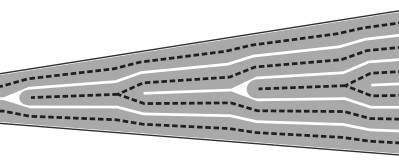
\includegraphics[width=\columnwidth]{sources/method/single_bead_strategy.jpg}
\caption{Overview}
\label{single_bead_strategy_overview}
\end{subfigure}
\begin{subfigure}{0.45\columnwidth}
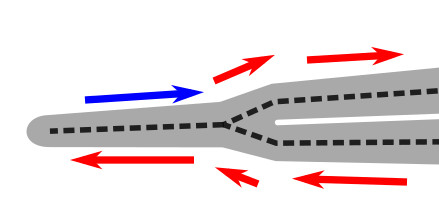
\includegraphics[width=\columnwidth]{sources/method/single_bead_strategy_order.jpg}
\caption{Travel order}s
\end{subfigure}
\caption{We can do single-bead segments. Blue is travel move.}
\label{single_bead_strategy}
\end{figure}

When all extrusion segments are generated, we combine them into semi-continuous polyline toolpaths.
These polylines generally form closed polygons, but at significant regions of the VQ the toolpaths consist of single bead polyline toolpaths.
See \cref{single_bead_strategy}.
These single bead polylines can connect to polygonal toolpaths and they can also meet each other at 3-way junctions.
We determine the printing order for all segments of a given bead index by minimizing the travel distance using a greedy path order optimizer.
\todo{[implementation needed!]}


In general the toolpath location should be centered on the middle of the bead.
However, when the bead width is smaller than the nozzle size we might want to offset the toolpath toward a previously printed bead.
That way the previously printed bead occludes part of the hole in the nozzle such that the unoccluded hole is as wide as the required bead width.
The printing order and the toolpath positioning of the beading strategy are therefore interrelated.

Around 3-way junctions we need to prevent overextrusion.
We need to reduce the extrusion amount after the first time we pass an intersection: commonly known as \emph{ghosting}.
See \cref{ghosting}.
In order to realize the reduction we remove a section from the extrusion bead up to a distance equal to the feature radius from the junction.


\begin{figure}
\centering
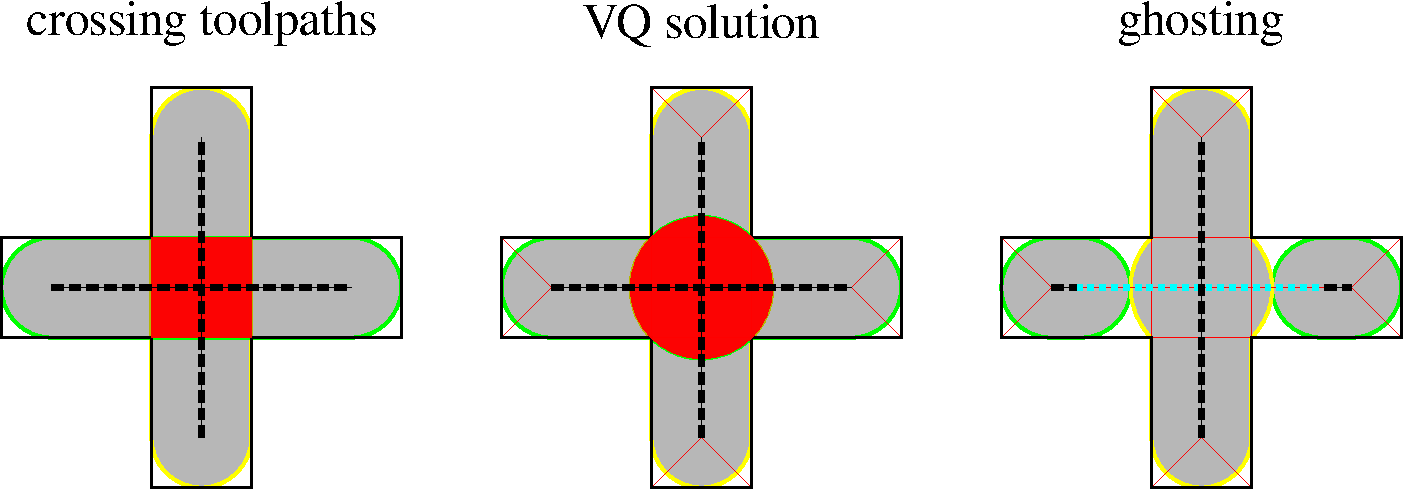
\includegraphics[width=.99\columnwidth]{sources/method/ghosting.pdf}
\caption{Ghosting prevents over-extrusion at junctions.}
\label{ghosting}
\end{figure}


























































